\chapter{Method}

\section{Step Detection}
\label{sec:meth - step detection}
The method used for step detection is similar to the one presented by \cite{Salvi2018}, introduced in \secref{sec:rw - step detection}. It differs from the referenced paper in that the data is being handled offline, not having to wait for data buffers to fill. It also differs in that it adds the walk detection method from \cite{Brajdic2013}. The values used for the different parameters are based on those found by \cite{Salvi2018}. The implemented method consists of five steps:
\begin{enumerate}
	\item \textbf{Pre-processing} \\
	The IMU used in most smartphones provide acceleration information over three orthogonal axes. For the step detection algorithm the magnitude of the combined signal from the three orthogonal axes is used. Since MEMS IMUs are subject to potential noise from different sources  the signal is put through a lowpass filter with a cutoff frequency of 5 hertz.
	
	\item \textbf{Walk detection} \\
	Since a person is not walking continuously, the regions in which it does occur need to be indicated. \cite{Brajdic2013} determined that thresholding on the standard deviation of the norm the accelerometer signal was sufficient. This is done using the parameters found by the paper, which is determining the standard deviation over a moving frame of 0.8 seconds, with all standard deviation magnitude levels above $0.6 m/s^2$ being considered walking.
	
	\item \textbf{Filtering} \\
	A gaussian window is applied with a window size of 13 frames and a standard deviation of 0.35.
	
	\item \textbf{Scoring }\\
	With the scoring stage the "peakiness" of a given sample is evaluated. The result
	of this stage should increase the magnitude of any peaks. This makes it easier for the subsequent peak detection. The scoring used is that of mean difference 
	\begin{equation}
		p_{i}=\frac{\sum_{k=-N, k \neq i}^{N}\left(x_{i}-x_{i+k}\right)}{2 N}
		\label{eq:mean difference}
	\end{equation}
	where $p$ is the score given to the sample, $i$ is the index of the sample, $N$ is window size, and $x$ is the sample value.
	
	
	\item \textbf{Step detection} \\
	Here outliers are statistically detected. The algorithm processes the signal by calculating a running mean and standard deviation.
	These two measures determine whether a sample is an outlier or not. If the difference between sample and mean is over 1.2 times the standard deviation, then it is marked as a potential step.
	
	
	\item \textbf{Post-processing} \\
	The final stage of step detection is determining local maxima of the outliers detected in the previous stage. Here local maxima are found that have a minimum separation duration of 0.2 seconds.
	
\end{enumerate}

An example of this step detection method and its different stages can be found in \cref{fig:all_stages_of_step_detection}.

\begin{figure}[H]
	\centering
	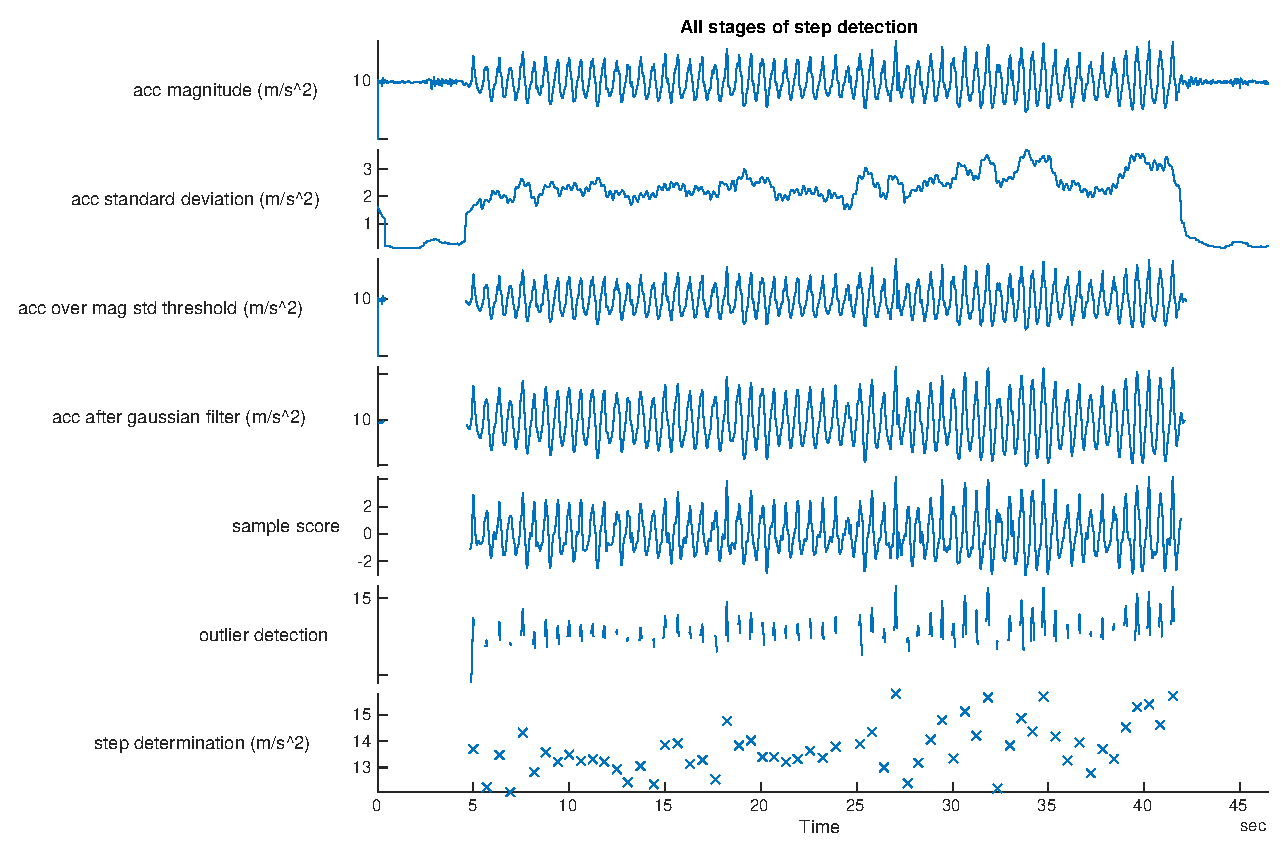
\includegraphics[width=1\linewidth]{images/20200924_1204_All_stages_of_step_detection}
	\caption[All stages of step detection ]{All stages of step detection from recorded accelerometer data, with the x's in the last graph indicating the steps taken }
	\label{fig:all_stages_of_step_detection}
\end{figure}

\section{Step Length Estimation}

\section{Orientation Estimation}
\subsection{Coordinate Frames}
Within orientation estimation there are  different coordinate frames to be considered. There are two frames that are of importance for localization: the body frame and the navigation frame.\\
The body frame ($b$) is the coordinate frame of the IMU, the origin of which is at the center of the triaxial accelerometers found in the device \cite{Kok2017}. The navigation frame ($n$) is the geographical frame in which the user is moving. It is also the frame in which we want to determine the pose, consisting of orientation and position, of the body frame. For a localization application it is considered stationary \cite{Kok2017}.
A superscript on a vector is used to indicate in which coordinate frame it is expressed. For example,
$x^n$ is the vector $x$ expressed in the navigation frame. A double superscript on any orientation mapping from one frame to another indicates from which frame to which frame the rotation is occurring. For example,
$R^{nb}$ is a rotation matrix that maps from the body frame to the navigation frame.


\subsection{Orientation Parametrization}
Rotation matrices $R \in \mathbb{R}^{3 \times 3}$ have the following properties:

\begin{equation}
	\label{eq:rot_mat_properties}
	R R^{\top}=R^{\top} R=I_{3}, \quad \text { det } R=1.
\end{equation}

These matrices can be used to express a vector $x$ in frame $v$ to frame $u$ as 

\begin{equation}
	\label{eq:rot_mat_rot_x}
	x^{\mathfrak{u}}=R^{\mathfrak{u} \mathrm{v}} x^{\mathrm{v}}.
\end{equation}

Transposing a rotation matrix represent a rotation back to it's original coordinate frame:
\begin{subequations}
	\begin{align}
		\label{eq:rot_mat_trans}
		x^{\mathrm{v}}&=\left(R^{\mathrm{uv}}\right)^{\top} x^{\mathrm{u}},\\
		&=R^{\mathrm{vu}} x^{\mathrm{u}}.
	\end{align}
\end{subequations}

A quarternion is a common parametrization of orientation frequently used by attitude estimation algorithms. This is because it is free of non-singularity in attitude representation \cite{Hashim2019}, also known as wrapping. A unit quaternion can be described by

\begin{equation}
	\label{eq:unit_quarternion}
	q=\left(\begin{array}{llll}{q_{0}} & {q_{1}} & {q_{2}} & {q_{3}}\end{array}\right)^{\top}
	=\left(\begin{array}{l}{q_{0}} \\ {q_{v}}\end{array}\right), 
	\quad q \in \mathbb{R}^{4}, 
	\quad\|q\|_{2}=1.
\end{equation}

A rotation of vector $x$ using quaternions between two frames, from $v$ to $u$, is indicated as

\begin{equation}
	\label{eq:quat_rot}
	\bar{x}^{\mathrm{u}}=q^{\mathrm{uv}} \odot \bar{x}^{\mathrm{v}} \odot q^{\mathrm{vu}},
\end{equation}

where $q^{\mathrm{vu}} = \left(q^{\mathrm{uv}}\right)^{\mathrm{c}}$, with the latter representing the quaternion conjugate, defined by 

\begin{equation}
	\label{eq:quat_conjugate}
	q^{\mathrm{c}}=\left(\begin{array}{c}{q_{0}} \\ {-q_{v}}\end{array}\right).
\end{equation}

$\bar{x}^u$ represents the quaternion version of the vector $x^u \in \mathbb{R}^3$, as

\begin{equation}
	\label{eq:quat_vec_ref}
	\bar{x}^u=\left(\begin{array}{l}{0} \\ {x^u}\end{array}\right).
\end{equation}


The $\odot$ operator describes quaternion multiplication, defined by:

\begin{equation}
	\label{eq:quat_multiplication}
	p \odot q=\left(\begin{array}{c}{p_{0} q_{0}-p_{v} \cdot q_{v}} \\ {p_{0} q_{v}+q_{0} p_{v}+p_{v} \times q_{v}}\end{array}\right)
\end{equation}

\subsection{Motion and Measurement Models}
\label{sec:motion_and_measurement_models}
The signals generated by an IMU can be formatted in such a way that orientation can be deduced. For many sensor fusion algorithms this is generally done by defining a motion and measurement model, together forming a state space representation. This state space can be defined as \cite{Kok2017}

\begin{subequations}
	\begin{align}
		\label{eq:orient_dynamics}
		q_{t+1}^{\mathrm{nb}} &=q_{t}^{\mathrm{nb}} \odot \exp _{\mathrm{q}}\left(\frac{T}{2}\left(y_{\omega, t}+e_{\omega, t}\right)\right), 	\\ 
		\label{eq:orient_acc_measure}
		y_{\mathrm{a}, t} &=-R_{t}^{\mathrm{bn}} g^{\mathrm{n}}+e_{\mathrm{a}, t},\\ 
		\label{eq:orient_mag_measure}
		y_{\mathrm{m}, t} &=R_{t}^{\mathrm{bn}} m^{\mathrm{n}}+e_{\mathrm{m}, t}, 
	\end{align}
	\begin{equation}
		\label{eq:orient_ss_noise}
		e_{\omega, t} \sim \mathcal{N}\left(0, \sigma_{\mathrm{\omega}}^{2} \mathcal{I}_{3}\right), 
		\quad 
		e_{\mathrm{a}, t} \sim \mathcal{N}\left(0, \sigma_{\mathrm{a}}^{2} \mathcal{I}_{3}\right), 
		\quad 
		e_{\mathrm{m}, t} \sim \mathcal{N}\left(0, \sigma_{\mathrm{m}}^{2} \mathcal{I}_{3}\right).
	\end{equation}
	\label{eq:orient_state_space}
\end{subequations}

Here \cref{eq:orient_dynamics} is the motion model and \cref{eq:orient_acc_measure,eq:orient_mag_measure} are the measurement models. \\
For the motion model, $q^{nb}$ represents unit quaternion from body $(b)$ to navigation frame $(n)$. $T$ is the time period between two samples. $y_{\omega, t}$ is the gyroscope measurement. The $\odot$ operator describes quaternion multiplication, as in \cref{eq:quat_multiplication}. The $\text{exp}_\text{q}$ operator is defined as

\begin{equation}
	\exp_\mathrm{q} (\eta) = \left(\begin{array}{c}{\cos \|\eta\|_{2}} \\ {\frac{\eta}{\|\eta\|_{2}} \sin \|\eta\|_{2}}\end{array}\right) \label{eq:exp_q_in_text}.
\end{equation}

For the measurement model, $y_{\mathrm{a}, t}\in \mathbb{R}^3$ is the accelerometer measurement and $R^\mathrm{nb}_t$ is the rotation matrix mapped from the orientation quaternion generated in \eqref{eq:orient_dynamics}. $g^n \in \mathbb{R}^3$ is the gravity vector in the navigation frame. Similarly, $y_{\mathrm{m}, t}\in \mathbb{R}^3$ is the accelerometer measurement and $m^n$ is the magnetic field in the navigation frame. \\
This state space model is simplified using certain assumptions.
For both motion and measurement models, the noise terms  $(e)$ is assumed to be normally distributed, independent and have the same noise levels for the three sensor axis of all three sensors, as indicated in \cref{eq:orient_ss_noise}. The zero mean in these noise definitions also indicate the assumption that the sensors have been calibrated properly and therefore do not contain any bias. \\
Another assumption is that the sensor does not travel over significant distances in comparison to the size of the earth \cite{Kok2017}. Additionally the magnitude of the earth rotation and coriolis acceleration are discarded. Furthermore, it is assumed that the acceleration signal is dominated by the gravity vector, making external acceleration negligible. Additionally, the magnetic field is assumed to be constant. These different assumptions will be needed to taken into account when constructing orientation estimation while walking indoors.

\subsection{Calibration}

For proper orientation estimation . \citet{Moder2017} indicates that it is  beneficial for PDR systems to have the gyroscope and magnetometer bias  calibrated, while the accelerometer bias and scale factor is optional. In addition it is advised to estimate the gyroscope bias frequently before testing.

\subsubsection{Gyroscope Calibration}
Gyroscope measurements from MEMS IMUs are generally offset by a bias ($o_\omega$) resulting in

\begin{equation}
	y_{\omega, t}=\omega_{t}+o_{\omega}+e_{\omega, t},
\end{equation}

where $e_{\omega, t}$ is assumed to have the same noise properties as in \cref{eq:orient_ss_noise}. The gyroscope bias is slowly time varying but for relatively short experiments can be assumed to be constant \cite{Kok2016}. It can be measured by placing the gyroscope on a flat surface for some time and recording data from the sensor. Since the sensor is not moving, the biases are the means of the data over the three axis and the covariance is the square of the standard deviation of the data to the previously mentioned means.

\subsubsection{Accelerometer and Magnetometer Calibration}
 In outdoor environments, mn is equal to the local earth magnetic field and is accurately
known from geophysical studies, see e.g. [29]. In indoor environments, however, the local magnetic
field can differ quite significantly from the local earth magnetic field. Because of that, we treat mn as
an unknown constant. 

For magnetometer and accelerometer calibration the method outlined by \citet{Kok2016} can be used. This method indicates that for a perfect calibration a magnetometer measures the local magnetic field, no matter the orientation. Any measurement will then lie on a sphere with a radius  equal to the local magnetic field. The same applies for a perfect calibration with an accelerometer, replacing the local magnetic field with the gravity vector. Any sensor calibration should strive to achieve this sphere as best as possible.\\
MEMS sensor are imperfect sensors, with sensor specific errors that can differ per sensor. These errors, including non orthogonality of sensor axis, the presence of zero bias, and difference in sensitivity on different axis \cite{Kok2016} can be combined into a distortion matrix $D$ and offset vector $o$.
This results in the following uncalibrated measurement model,
\begin{equation}
	y_{\mu, t}=D_\mu R_{t}^{\mathrm{bn}} \mu^{\mathrm{n}}+o_\mu +e_{\mu, t},
\end{equation}

where $\mu$ is a placeholder for either the acceleration vector or local magnetic field vector with the superscript indicating in what coordinate frame it is expressed. Each have their own respective distortion matrix and offset vector. $y_{\mu, t}$ represents the measurement associated with either gyroscope or magnetometer.
Due to the distortion matrix and offset vector, the measurements lie on a translate ellipsoid instead of on a sphere as previously stated. Determining these parameters, the sensor errors can be compensated through

\begin{equation}
	y_{\mu, t}^{cal}=D_\mu^{-1}\left(y_{\mu, t}-o_{\mu}\right)
\end{equation}

Without loss of generality the desired sphere radius can be normalized and written as followed to expressed the sphere characteristic
\begin{equation}
	\begin{aligned}
		\left\|\mu^{\mathrm{b}}\right\|_{2}^{2}-1 &=\left\|R_{t}^{\mathrm{bn}} \mu^{\mathrm{n}}\right\|_{2}^{2}-1 \\
		&=\left\|D^{-1}\left(y_{\mu, t}-o-e_{\mu, t}\right)\right\|_{2}^{2}-1=0.
	\end{aligned}
\end{equation}

Since real calibration measurements are still corrupted by noise, the above equality does not hold exactly. The ellipsoid fitting problem can be rewritten as

\begin{equation}
	\label{eq:calib_elipsoid}
	y_{\mu, t}^{\top} A y_{\mu, t}+b^{\top} y_{\mu, t}+c \approx 0,
\end{equation}
where
\begin{subequations}
	\label{eq:calib_elipsoid_components}
	\begin{align}
		A \triangleq D_\mu^{-\top} D_\mu^{-1}, \\
		b \triangleq-2 o_\mu^{\top} D_\mu^{-\top} D_\mu^{-1}, \\
		c \triangleq o_\mu^{\top} D_\mu^{-\top} D_\mu^{-1} o_\mu.
	\end{align}
\end{subequations}

Assuming that $A$ is positive definite, this defines an ellipsoid with parameters $A, b$ and $c$. This can be rewritten as a linear relation as

\begin{equation}
	M \xi \approx 0
\end{equation}
with
\begin{equation}
	M=\left(\begin{array}{ccc}
		y_{\mu, 1} \otimes y_{\mu, 1} & y_{\mu, 1} & 1 \\
		y_{\mu, 2} \otimes y_{\mu, 2} & y_{\mu, 2} & 1 \\
		\vdots & \vdots & \vdots \\
		y_{\mu, N} \otimes y_{\mu, N} & y_{\mu, N} & 1
	\end{array}\right), \quad \xi=\left(\begin{array}{c}
		\mathrm{vec} A \\
		b \\
		c
	\end{array}\right),
\end{equation}

where $\otimes$ is the kronecker product and vec the vectorization operator.
The ellipsoid fitting problem can be written as the following semidefinite program \cite{Kok2016} 
\begin{equation}
	\begin{array}{ll}
		\min _{A, b, c} & \frac{1}{2}\|M\left(\begin{array}{c}
			\operatorname{vec} A \\
			b \\
			c
		\end{array}\right)\|_{2}^{2} \\
		\text { s.t. } & \operatorname{Tr} A=1, \quad A \in S_{++}^{3 \times 3}
	\end{array},
\end{equation}

where $S_{++}^{3 \times 3}$ is the set of $3 \times 3$ positive definite symmetric matrices. This is a convex optimization problem with a globally optimal solution that can be solved using software packages such as CVX \cite{cvx} and YALMIP \cite{Lofberg2004}. Initial estimates of the calibration matrix $D_\mu$ and offset vector $o_\mu$ can be obtained from the estimated $\widehat{A}, \widehat{b}, \widehat{c}$ defined as

\begin{subequations}
	\begin{align}
		\beta &=\left(\frac{1}{4} \hat{b}^{\top} \widehat{A}^{-1} \widehat{b}-\widehat{c}\right)^{-1} \\
		\widetilde{D}_{\mu 0}^{\top} \widetilde{D}_{0} &=\beta \widehat{A}^{-1} \\
		\widehat{o}_{\mu 0} &=\frac{1}{2} \widehat{A}^{-1} \widehat{b}
	\end{align}
\end{subequations}

An example of this calibration can be found in \cref{fig:calibration_magnetometer} where data was recorded by recording a smartphone in as many orientations as possible, in a stationary setting. It clearly shows how the uncalibrated data is mapped to a unit sphere. The distortion matrix and offset vector for this calibration are 

\begin{subequations}
	\begin{align}
	\widehat{D}_{m0} &= \left(\begin{array}{rrr}
		0.0203 & -0.0001 & -0.0009 \\
		0 & 0.0191 & 0.0000 \\
		0 & 0 & 0.0199
	\end{array}\right), \\
	\widehat{o}_{m0} &= \left(\begin{array}{r}
		-13.3918 \\
		81.0407 \\
		20.9336
	\end{array}\right).
	\end{align}
	
\end{subequations}

\begin{figure}[H]
	\centering
	\begin{subfigure}[t]{.4\textwidth}
		\centering
		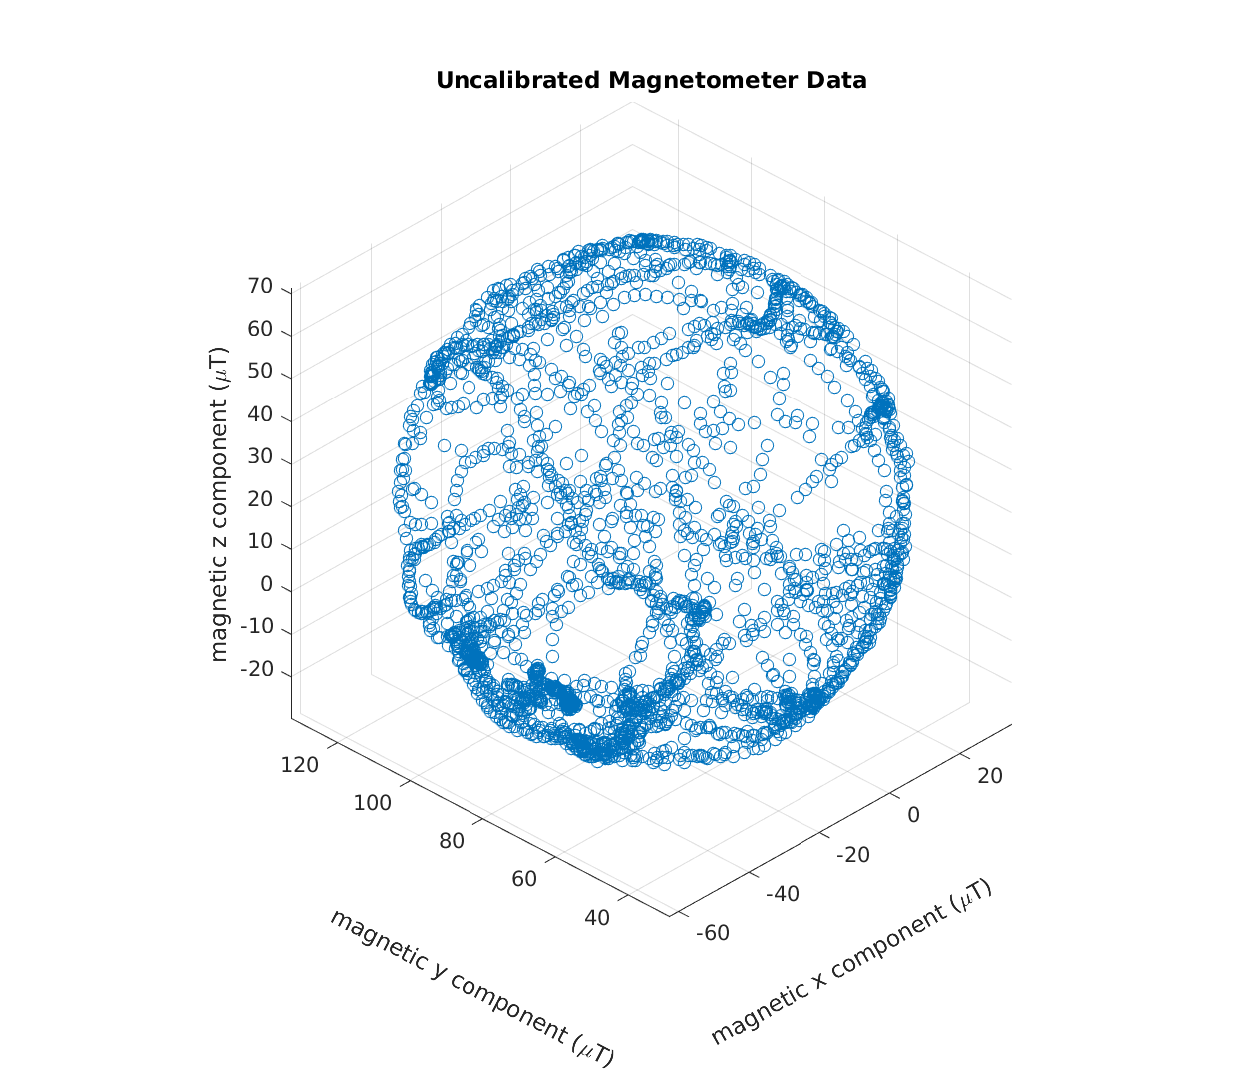
\includegraphics[width=\linewidth]{images/20201020_1125_Uncalibrated_Magnetometer_Data}
		\caption{Uncalibrated magnetometer data}
		\label{fig:uncalibrated_magnetometer_data}
	\end{subfigure}
	\begin{subfigure}[t]{0.4\textwidth}
		\centering
		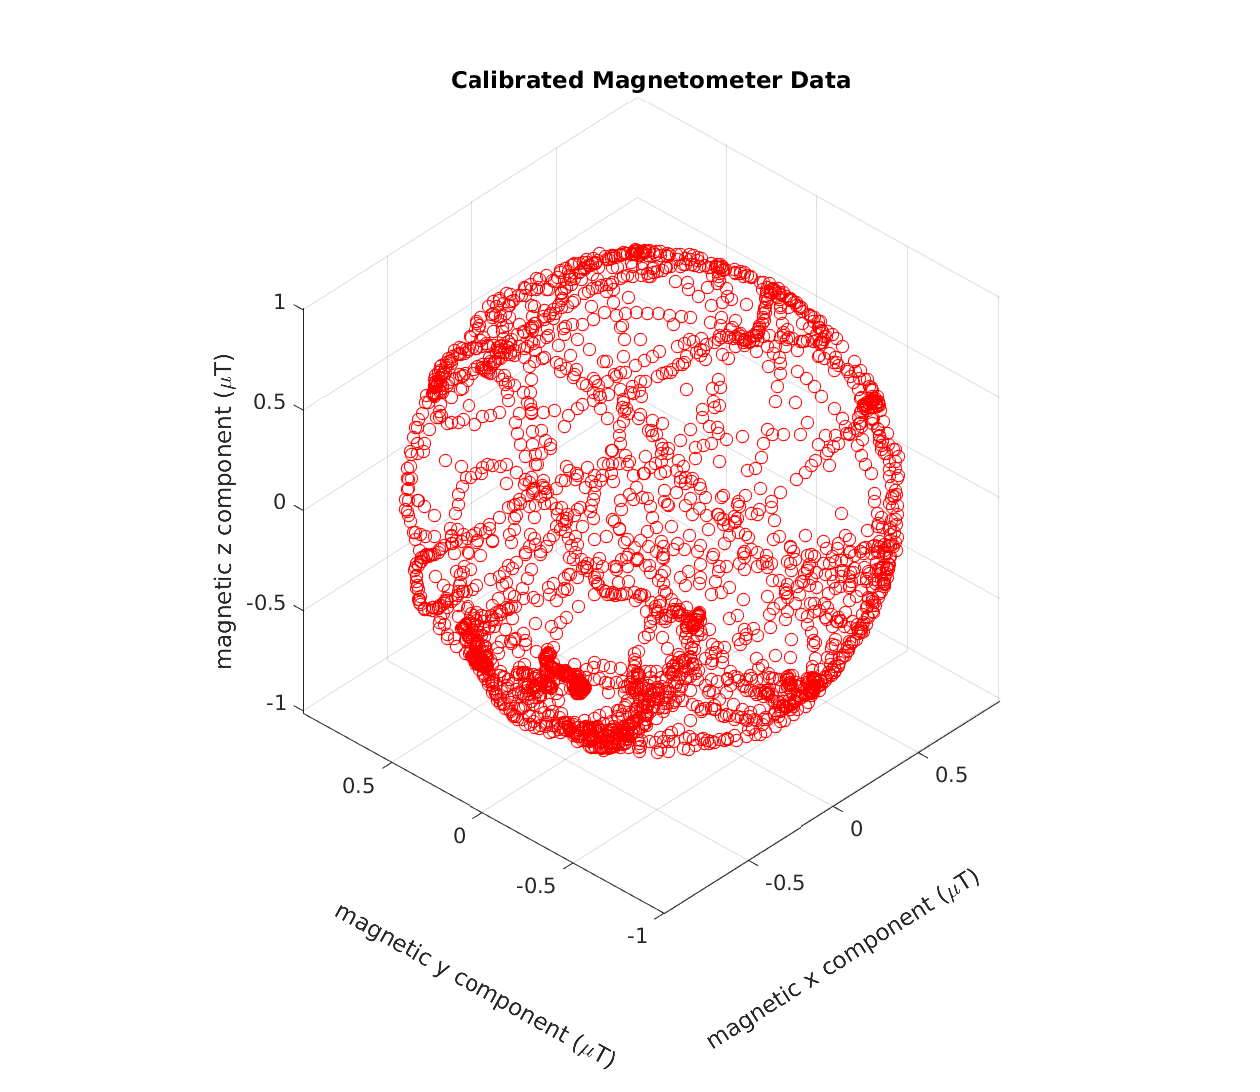
\includegraphics[width=\linewidth]{images/20201020_1125_Calibrated_Magnetometer_Data}
		\caption{ Calibrated magnetometer data}
		\label{fig:calibrated_magnetometer_data}
	\end{subfigure}
	\caption{Magnetometer calibration for smart MEMS IMU in one location}
	\label{fig:calibration_magnetometer}
\end{figure}


\subsection{Extended Kalman Filter}
\label{sec:method-EKF}
The Kalman Filter (KF) uses a linear state space model in combination with measurements and its characteristics to make an unbiased minimum-variance estimator \cite{verhaegen2007filtering}. The KF assumes that the noise affecting the state space model is additive and that both process and measurement noise are Gaussian and zero mean.
The Kalman Filter consists of three steps, with the last two steps performed recursively. The first is stating an initial estimate and the variance of the process and measurement noise.  The second is the time update in which the state is propagated through a motion model, which may or may not have an external input, resulting in a one step ahead estimate. The third step is the measurement update in which the estimate generated by the time update is compared with actual measurements related to the state being estimated. Discrepancies between the two will lead to an error measurement. This error can then be used to correct the estimate.
The Extended Kalman Filter (EKF) is an adaptation of the Kalman Filter that estimates for non linear models. 

For orientation estimation the motion and measurement model presented in \cref{eq:orient_state_space} can be used. As stated in \cref{sec:motion_and_measurement_models}, this model has assumptions that need to be accommodated. This will have to be incorporated in the EKF. Additionally sensor data does not all arrive at the same time. This means that the measurement update will potentially need to only update with either magnetometer or accelerometer data.  

\subsubsection{Time Update}

A time update occurs every time a gyroscope measurement ($y_\omega$) is received. It calculates a one step ahead estimate of the state vector and its covariance matrix. The calculations are as followed: 

\begin{subequations}
\begin{align}
\hat{q}_{t | t-1}^{\mathrm{nb}}=\hat{q}_{t-1 | t-1}^{\mathrm{nb}} \odot \exp _{\mathrm{q}}\left(\frac{T}{2} y_{\omega, t-1}\right) \\
P_{t | t-1}=F_{t-1} P_{t-1 | t-1} F_{t-1}^{\top}+G_{t-1} Q G_{t-1}^{\top}
\end{align}
with $Q = \Sigma_\omega$ and $P$ the state covariance. Here
\begin{align}
F_{t-1}&=\left(\exp _{q}\left(\frac{T}{2} y_{\omega, t-1}\right)\right)^{R},\\
G_{t-1}&=-\frac{T}{2}\left(\hat{q}_{t-1 | t-1}^{\mathrm{nb}}\right)^{L} \frac{\partial \exp _{q}\left(e_{\omega, t-1}\right)}{\partial e_{\omega, t-1}},
\end{align}
\end{subequations}
where $q^L$ and $q^R$ are defined as 
\begin{subequations}
\begin{equation}
q^L = \left(\begin{array}{cc}{q_{0}} & {-q_{v}^{\top}} \\ {q_{v}} & {q_{0} \mathcal{I}_{3}+\left[q_{v} \times\right]}\end{array}\right),
\end{equation}	
\begin{equation}
q^R = \left(\begin{array}{cc}{q_{0}} & {q_{v}^{\top}} \\ {-q_{v}} & {q_{0} \mathcal{I}_{3}+\left[q_{v} \times\right]}\end{array}\right).
\end{equation}
\end{subequations}

\subsubsection{Measurement Update}

A measurement update occurs every time either an accelerometer or magnetometer reading is received. \\
To ensure that the assumptions of the gravity vector being dominant in the accelerometer and the homogeneous magnetic field being dominant in the magnetometer, thresholds can be used. This is of importance with pedestrian dead reckoning, as a walking motion will induce additional external forces, affecting the acceleration measured by the IMU. Additionally, when localizing indoors, magnetic disturbance within the built environment will affect the magnetometer readings.\\
The measurement update for the EKF with quaternions as states is as followed:

\begin{subequations}
	\begin{align}
	\tilde{q}_{t | t}^{\mathrm{nb}} &=\hat{q}_{t | t-1}^{\mathrm{nb}}+K_{t} \varepsilon_{t}, \\
	\tilde{P}_{t | t} &=P_{t | t-1}-K_{t} S_{t} K_{t}^{\top}
	\end{align},
	with	
	\begin{align}
	\varepsilon_{t} &= y_{t}-\hat{y}_{t | t-1},\\
	\quad S_{t} &= H_{t} P_{t | t-1} H_{t}^{\top}+R, \\
	\quad K_{t} &= P_{t | t-1} H_{t}^{\top} S_{t}^{-1}.
	\end{align}
\label{eq:quat_meas_update}	
\end{subequations}


If an accelerometer measurement is received and whos magnitude falls in an interval around the magnitude , the variables to use in \cref{eq:quat_meas_update} are

\begin{subequations}
	\begin{align}
	y_{t}&=
	y_{\mathrm{a}, t}, \\
	\hat{y}_{t | t-1}&=
	-\hat{R}_{t | t-1}^{\mathrm{bn}} g^{\mathrm{n}},\\
	H_{t}&=	-\left.\frac{\partial R_{t | t-1}^{\mathrm{bn}}}{\partial q_{t | t-1}^{\mathrm{nb}}}\right|_{{q_{t | t-1}^{\mathrm{nb}}}=\hat{q}_{t | t-1}^{\mathrm{nb}}} \quad g^{\mathrm{n}}.
	\end{align}
\end{subequations}

Likewise if a magnetometer measurement arrives and meets the threshold requirement, the variables are defined as

\begin{subequations}
	\begin{align}
	y_{t}&=	y_{\mathrm{m}, t},\\
	\hat{y}_{t | t-1}&=	\hat{R}_{t | t-1}^{\mathrm{bn}} m^{\mathrm{n}},\\
	H_{t}&=	\left.\frac{\partial R_{t | t-1}^{\mathrm{bn}}}{\partial q_{t | t-1}^{\mathrm{nb}}}\right|_{{q_{t | t-1}^{\mathrm{nb}}}=\hat{q}_{t | t-1}^{\mathrm{nb}}} \quad m^{\mathrm{n}}.
	\end{align}
\end{subequations}

\subsubsection{Renormalization}
Once a measurement update occurs the resulting quaternion is not necessarily a unit quaternion, which is a requirement for orientation parametrization. To facilitate this a renormalize the quaternion is required, using

	\begin{equation}
	\hat{q}_{t | t}^{\mathrm{nb}}=\frac{\tilde{q}_{t-1}^{\mathrm{nb}}}{\left\|\tilde{q}_{t | t}^{\mathrm{nb}}\right\|_{2}}.
	\end{equation}

Using steps outlined in \cite{Kok2017} and \cite{Linkoping2013}, the above outlined EKF was implemented in MATLAB. It was preliminarily  tested in a limited case with actual smartphone sensors. Calibration and testing occurred in the same room, where the phone was continuously randomly orientated while recording sensor data. This data was afterwards exported and entered into the EKF. The results can be seen in \cref{fig:simple_stationary_ekf}, where it is compared with the orientation estimation calculated by the android system. It is clear that the orientation estimation is almost identical to the system derived orientation.

\begin{figure}[H]
	\centering
	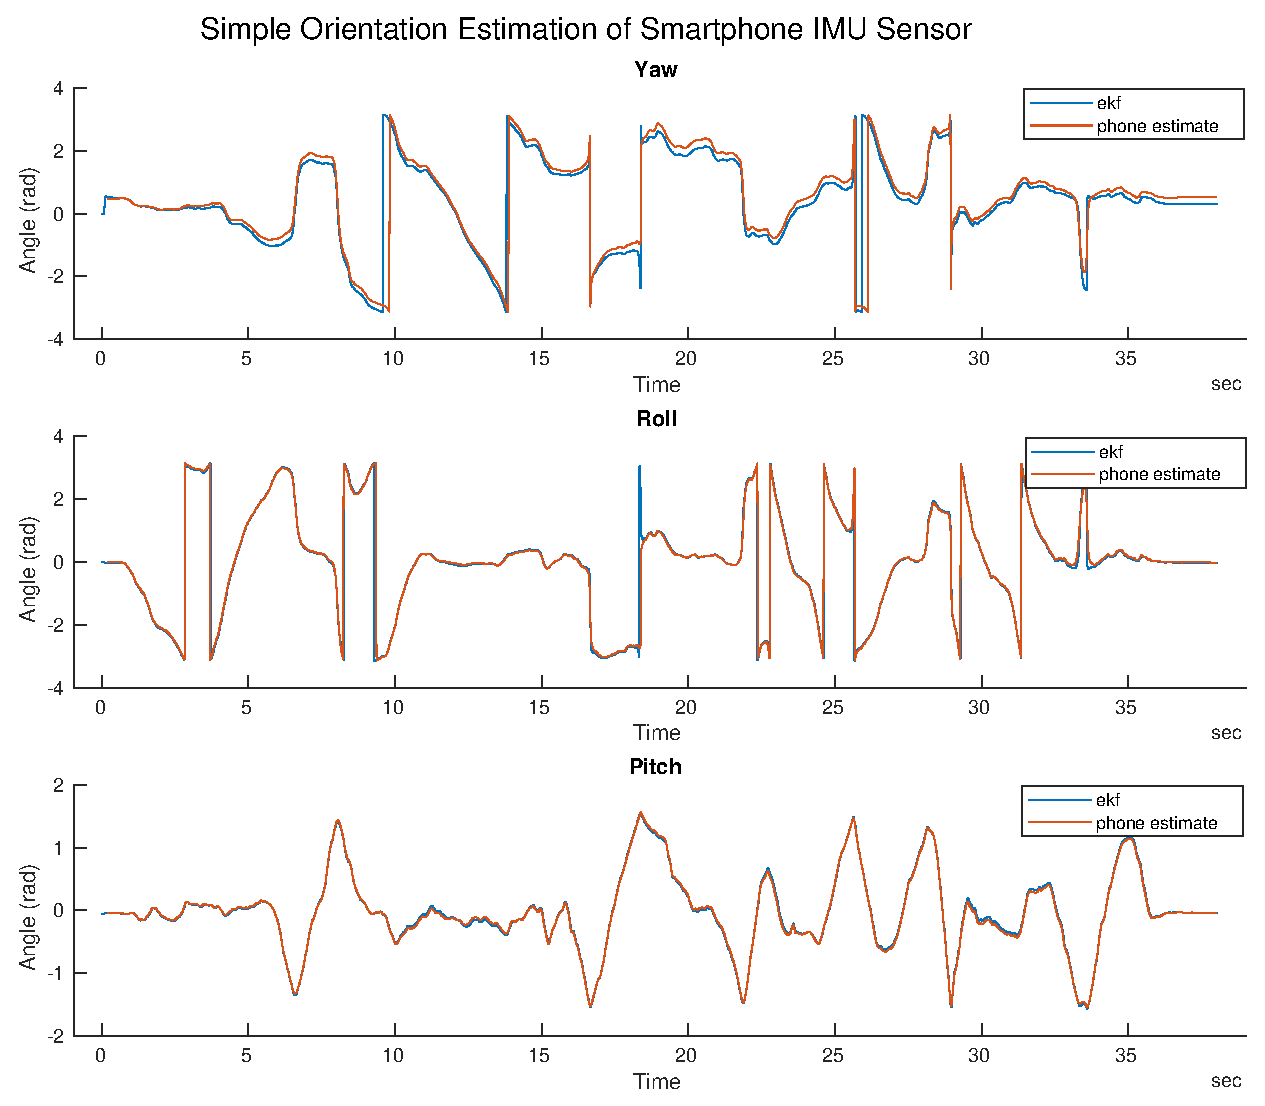
\includegraphics[width=0.7\linewidth]{images/20201025_2015_simple_stationary_ekf}
	\caption[Simple orientation estimation comparison]{ Simple orientation estimation comparison between own EKF and android orientation estimation}
	\label{fig:simple_stationary_ekf}
\end{figure}

\newpage
\section{Particle Filter}
\label{sec:method-pf}
The step and heading system,which combines step detection and length estimation with orientation estimation, generates an estimate of the trajectory walked by the pedestrian. Since there are uncertainties in all aspects of the SHS, it is inevitable that drift will occur within. The estimate then no longer accurately represents reality. In order to counter this drift, one method is to use map information in combination with a Particle Filter. This is a numerical Bayes estimator able to estimate non linear posterior densities, allowing for multimodal distributions \cite{gustafsson2010particle,kihlberg2012map}. Multimodal distribution refers to distributions with multiple maxima in the probability density function. This allows the particle filter to have multiple hypothesis for the system that it is modeling. In the case of localization, it may therefore indicate that there are two position estimates are equally as likely based on the information that the filter has received so far. This can occur due to symmetry in the indoor environment \cite{Woodman2008}. \\
The particle filter is known to work well in three dimensional state space \cite{gustafsson2010particle}, with higher dimensions making the particle representation too sparse to be a meaningfully represent the posterior distribution. Since for indoor localization only y position, x position and heading are needed, the particle filter is sufficient.
\par
As the name suggests, the particle filter uses a finite amount of particles to determine a state estimate. These particles are weighted and are propagated through a motion model, augmented with a noise realization on relevant variables. These noise realizations represent uncertainty of certain components of the motion model. The probability density function of these noise realizations are defined beforehand. Taking the weighting of each particle into account a prior estimate can be made. The particle cloud is then, when possible, compared with measurements, adjusting the weightings accordingly. These measurements may come from different sources. This process is familiar to the reader as it closely resembles that of the previously mentioned Kalman Filter, also a Bayes estimator.\par
For indoor localization on one floor the state space is defined as $\mathbb{R}^{2}$, and in combination with map information is limited by the outer perimeter of the building the user is located in. The particle is defined by 

\begin{equation}
x_k^i = \left(\begin{array}{l}
x \; position \\
y \; position\\
heading
\end{array}\right), 
\label{eq:pf_state}
\end{equation}
where $x^i_k$ is the state of particle $i$ at time $k$.\\
The initialization of the particle cloud depends on information known beforehand. If there is a known initial position, all particles can be initialized around that point. Otherwise the particles can be initialized by spreading them evenly within the outer perimeter of the building. The initial weight of  once initialized the following four steps are performed recursively \cite{Wu2019,Woodman2008}: 

\begin{enumerate}
	\item \textbf{Measurement update} \\
	Each particle is weighted against constraints or system evaluation function. The likelier the particle is within the system constraints, the higher the weighting is. Each particle weighted is redefined through
	\begin{subequations}
		\begin{equation}
		\omega^i_{k} = \frac{1}{c_k} \omega^i_{k-1} p(y_k|x^i_k),
		\end{equation}\\
		where the normalization weight ($c_k$) is given by
		\begin{equation}
		c_{k}=\sum_{i=1}^{N} w_{k-1}^{i} p\left(y_{k} | x_{k}^{i}\right)
		\label{eq:PF_probability density}
		\end{equation}
	\end{subequations}
	
	
	Here $\omega^i_k$ is the weighting for particle $i$ at time $k$, $y_k$ is the measurement at time $k$,  and $N$ is the total number of particles. For localization, the state of the particle is its xy position. With a map, the position of physical structures can be compared with the trajectory of particles as a measurement. For example, if these structures cannot be traversed, as is the case with walls, the trajectory of a particle that crosses this structure is incorrect. Regions in which the user cannot be found have a likelihood of 0, while all indoor accessible regions have a likelihood of 1. This form of measurement turns wall information into a two dimensional probability density function, an example of which can be found in \cref{fig:pf_walls}.\par
	A map can also be used to compare particle position with landmark position of detectable activities. For example, maps indicate where doors are located. If a door opening activity can be detected a conditional probability can be used to determine the weighting of each particle. This conditional probability can be a multivariate normal probability density function. This is defined by a mean in x and y position, which is the xy position of each particle, and a standard deviation along both axis. This is shown visually by \cref{fig:pfdiagram}. Here there are three particles each with a multivariate normal probability density function represented by the different colored circle, with a gradient in opacity. The more opaque the higher the likelihood is. When compared to the position of the door the weight of particle P3 and P2 will be higher than that of P2. If a door activity is detected the weighting of P1 and P3 will be higher than P2. This increases the likelihood of these two particles being resampled in the next step. 
	
	\begin{figure}[H]
		\centering
		\begin{subfigure}[t]{.4\textwidth}
			\centering
			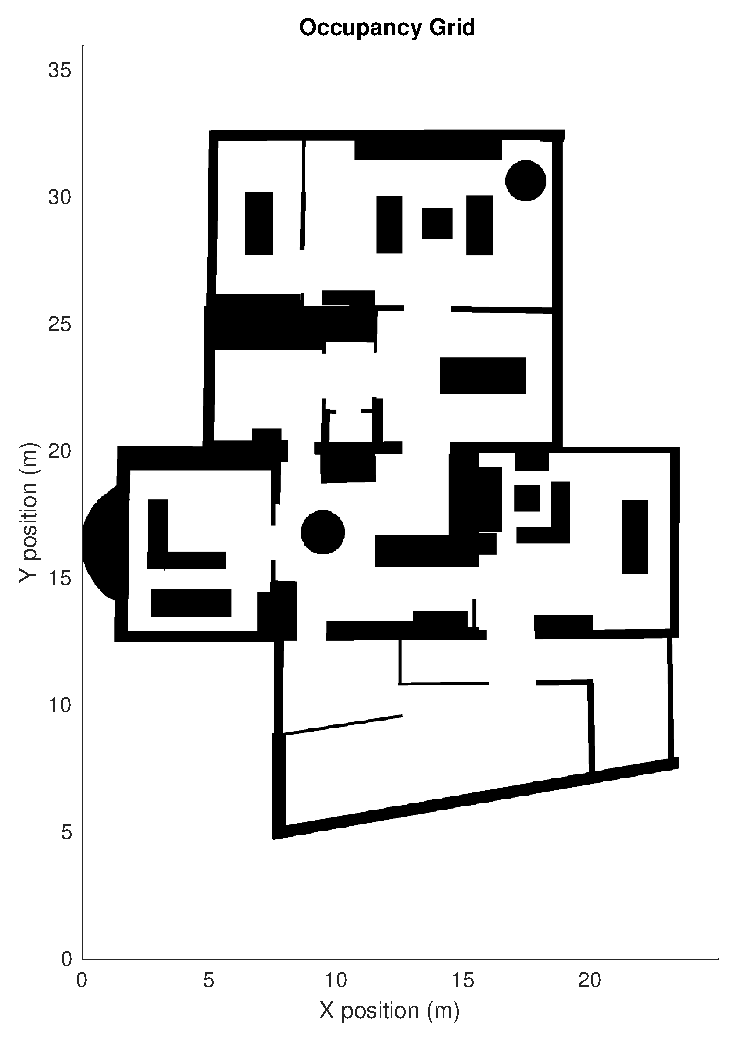
\includegraphics[width=0.7\linewidth]{images/20201030_1157_pf_map_1}
			\caption{2D probability density function from map information. black is zero likelihood and white is a likelihood of one.}
			\label{fig:pf_walls}
		\end{subfigure} \quad
		\begin{subfigure}[t]{0.4\textwidth}
			\centering
			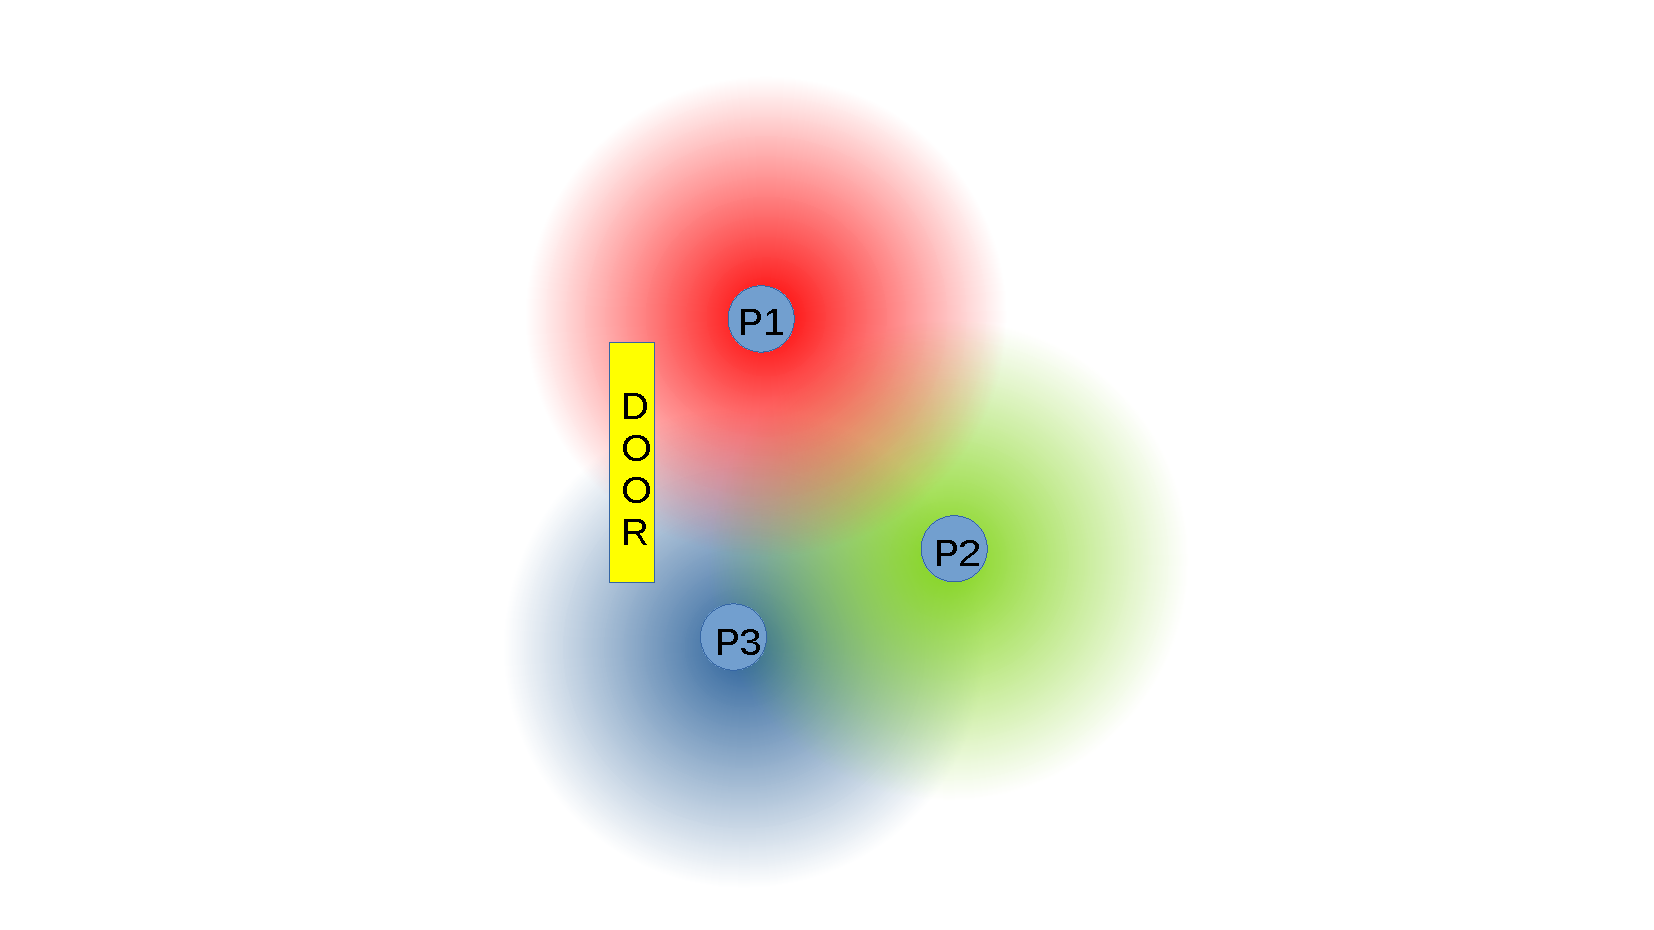
\includegraphics[trim=240 0 220 0, clip, width=0.7\linewidth]{images/pf_diagram}
			\caption{ Particles with a multivariate normal probability density function to determine weighting depending on position of a door}
			\label{fig:pfdiagram}
		\end{subfigure}
		\caption[Map information use in Particle Filter]{Map information for measurement updates in the particle filter}
		\label{fig:pf_meas_update}
	\end{figure}
	
	\item  \textbf{Estimation} \\
	Using the weightings and positions of the particle cloud, an estimate can be made of the posterior probability density of the process that is being modeled  \cite{gustafsson2010particle}. There a different ways of defining the. The maximum a posteriori (MAP) estimate picks the particle with the highest weight from the posterior probability function \cite{Saha2009}, while the  minimum mean square error (MMSE) estimate calculates a weighted mean \cite{gustafsson2010particle,Saha2009} as
	\begin{equation}
	\hat{x}_{k | k} =\sum_{i=1}^{N} w_{k}^{i} x_{k}^{i}.
	\end{equation}
	
	\item \textbf{Resampling}\\
	Depending on the new weights of the different particles, a subset is taken and resampled to form a new set of particles, which will be used in the next iteration of the particle filter. There a multiple methods that can be used for resampling including multinomial, stratified resampling, systematic resampling, and	residual resampling \cite{hol2006resampling}. \citet{hol2006resampling} conclude that from this set systematic resampling is the best considering resampling quality and computational complexity. For systematic resampling
	\begin{subequations}
		\begin{equation}
		x^{i*} = x(F^{-1}(u^i)),
		\end{equation}
		\begin{equation}
		u^i = \frac{(i-1) + \tilde{u}}{N}, \tilde{u} \sim \mathcal{U}[0,1).
		\end{equation}
	\end{subequations}
	
	Here $x^{i*}$ represents the newly sample particle with index $i$ and $F^{-1}$ represents the generalized inverse of the cumulative probability distribution of the normalized particle weights, $N$ is the total number of particles. \par
	Resampling inevitably destroys information and therefore increases uncertainty by the random sampling \cite{gustafsson2010particle}. Resampling should therefore occur only when it is needed. \citet{gustafsson2010statistical} proposes the use of  \textit{effective number of samples} to trigger a  resampling. This can be calculated as 
	\begin{subequations}
		\begin{equation}
		N_{\mathrm{eff}}=\frac{1}{\sum_{i=1}^{N}\left(w^{i}\right)^{2}},
		\end{equation}
		
		where
		
		\begin{equation}
		1 \leq N_{\mathrm{cff}} \leq N.
		\end{equation}
	\end{subequations}
	
	The resampling condition can then be defined as $N_{eff} < N_{th}$ \cite{gustafsson2010statistical}, where the threshold can be placed at $N_{th} = 2N/3$, with $N$ being the total number of particles.
	
	
	\item \textbf{Time update} \\	
	Each time step, every particle updates its own state with a dynamic model. For SHS, the dynamic model used is
	
	\begin{equation}
	\label{eq:SHS_dynamic_model_with_noise}
	x^i_{t + 1}
	=
	\left(\begin{array}{l}
	x(0)_{t} + (l_{t} + e_l) * \cos (x(2)_{t}) \\
	x(1)_{t} + (l_{t} + e_l) * \sin (x(2)_{t}) \\
	x(2)_{t} + \Delta \theta_t + e_\theta 
	\end{array}\right), \quad
	e_{\theta} \sim \mathcal{N}\left(0, \sigma_{\theta}^{2}\right), \quad e_{l} \sim \mathcal{N}\left(0, \sigma_{l}^{2}\right).
	\end{equation}
\end{enumerate}

where $x(*)$ indicates the index of the state vector defined in \cref{eq:pf_state}. The inputs to this dynamic model are $l_{t}$, which is the step length found by step detection and step length estimation, and $\Delta \theta_t$, which is the change in heading between the current and previous time step, found through the orientation estimation in \cref{sec:method-EKF}.

\section{Activity Recognition}